%-------------------------------------------------------
\begin{frame}{Introduction}{What is Data Mining?}
%-------------------------------------------------------

\noindent\begin{centering}
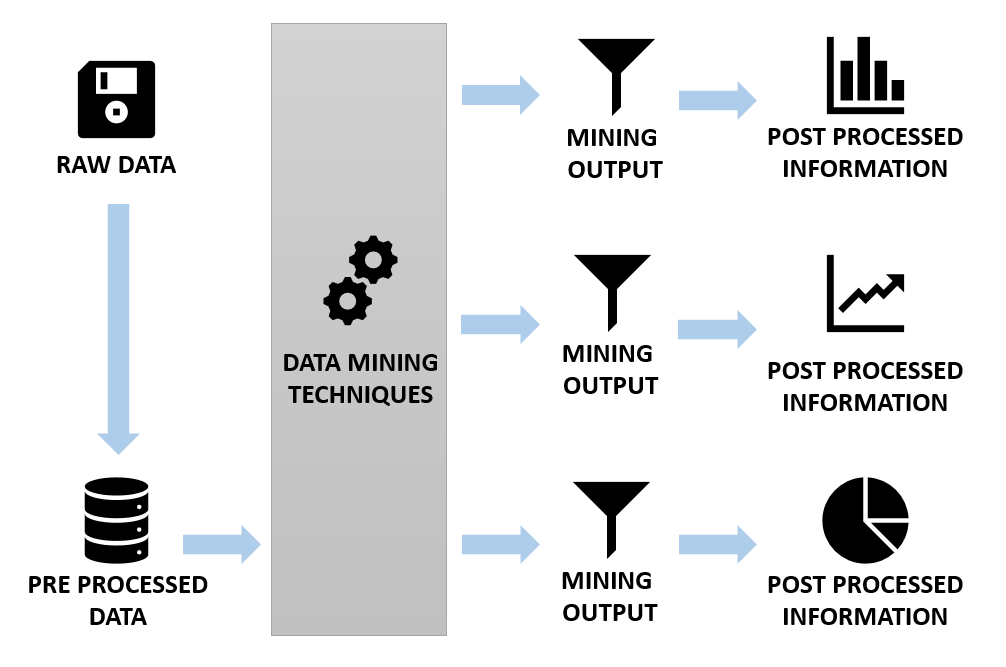
\includegraphics[scale=0.32]{img1_noback.png}
\end{centering}

\end{frame}

%-------------------------------------------------------
\begin{frame}{Introduction}{A general view about the Data Mining process}
%-------------------------------------------------------

    \centering\textit{What needs to be done?} \vspace{0,3cm}

	\begin{block}{}
		\begin{itemize}
			\item<1-> \textbf{Data Understanding}: analyze available raw data to \emph{understand} what can be extracted;
			\item<2-> \textbf{Preprocessing}: transform raw data into a \emph{minable} form, ready to be fed to the \emph{data mining algorithm};
			\item<3-> \textbf{Data Mining}: run the appropriate algorithm on the preprocessed data, to dig it for \emph{information};
			\item<4-> \textbf{Postprocessing}: display information in a human-friendly way, emphatizing what has beed dug with \emph{visualization technoques}.
		\end{itemize}
	\end{block}

\end{frame}

%-------------------------------------------------------
\begin{frame}{Introduction}{The choice of appropriate technologies}
%-------------------------------------------------------

	\centering\textit{Which technology should be employed?} \vspace{0,3cm}

	\begin{block}{}
	    \begin{itemize}
		    \item<1-> \alert{Data Processing} --- \textbf{MongoDB}: advanced \emph{dbms}, operating in the \emph{noSQL} paradigm.
		    \item<2-> \alert{Data Mining Algorithms} --- \textbf{Weka}: software which provide a \emph{framework} for running data mining algorithms.
			\item<3-> \alert{Visualization Techniques} \\
			--- \textbf{R language}: programming language which an extensive data visualization library; \\
			--- \textbf{Spreadsheets}: tabular data managing software, like Microsoft Excel and OpenOffice Calc.
	    \end{itemize}
    \end{block}

\end{frame}
